\documentclass{standalone}
\usepackage{tikz}
\usepackage{pgfplots}
\pgfplotsset{compat=newest}
\usepackage{amsmath}
\usepackage[american]{circuitikz}
\usepackage{cmbright}

\definecolor{myred}{RGB}{170,0,0}
\definecolor{myblue}{RGB}{0,0,220}
\definecolor{mygreen}{RGB}{0,150,0}
\definecolor{myorange}{RGB}{255,127,0}
\definecolor{mybrown}{RGB}{150,75,0}

\begin{document}
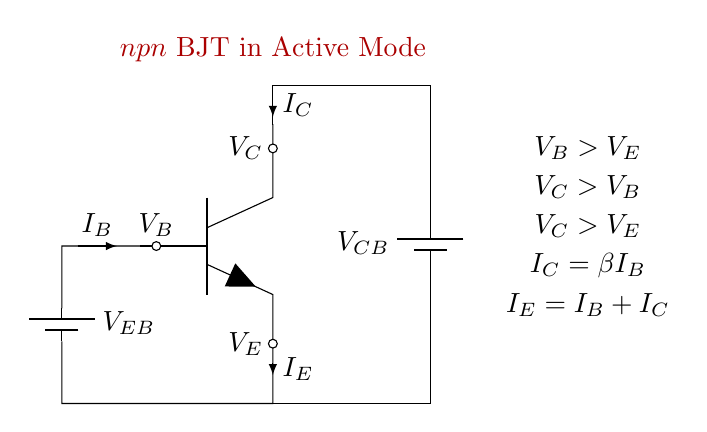
\begin{tikzpicture}
    \begin{scope}
        % Title
        \node[anchor=center, color=myred] at (0, 2.5) {$npn$ BJT in Active Mode};
        % npn BJT sumbol
        \draw (0, 0) node[npn, scale=2.0] (Q) {};
        \draw (Q.base) 
            to ++(-1, 0)
            to[battery1, l=$V_{EB}$] ++(0, -2)
            to ++(2.68, 0)
            to (Q.emitter);
        \draw (Q.collector)
            to ++(0, 0.5)
            to ++(2, 0)
            to[battery1, l_=$V_{CB}$] ++(0, -4.04)
            to ++(-2.0, 0);
        % Current arrows
        \draw[-latex, thin] (Q.base) ++(-0.8, 0.0) -- ++(0.5, 0) node[above, midway] {$I_B$};
        \draw[latex-, thin] (Q.emitter) ++(0.0, -0.1) -- ++(0, 0.15) node[midway, right] {$I_E$};
        \draw[-latex, thin] (Q.collector) ++(0, 0.4) -- ++(0, -0.3) node[midway, right] {$I_C$};
        % Add the transistor nodes.
        \node[ocirc] at ($(Q.base) + (0.2, 0)$) {};
        \node[anchor=south] at ($(Q.base) + (0.2, 0)$) {$V_B$};
        \node[ocirc] at ($(Q.emitter) + (0, 0.3)$) {};
        \node[anchor=east] at ($(Q.emitter) + (0, 0.3)$) {$V_E$};
        \node[ocirc] at ($(Q.collector) + (0, -0.3)$) {};
        \node[anchor=east] at ($(Q.collector) + (0, -0.3)$) {$V_C$};
    \end{scope}
    \begin{scope}[xshift=4cm]
        \path (0, 1.25) node[anchor=center, color=black] {$V_B > V_E$}
            ++(0, -0.5) node[anchor=center, color=black] {$V_C > V_B$}
            ++(0, -0.5) node[anchor=center, color=black] {$V_C > V_E$}
            ++(0, -0.5) node[anchor=center, color=black] {$I_C = \beta I_B$}
            ++(0, -0.5) node[anchor=center, color=black] {$I_E = I_B + I_C$};
    \end{scope}
\end{tikzpicture}
\end{document}